%\documentclass{book}
%\begin{document}
\chapter{Introduction}
\lhead{Chapter 1. \emph{Introduction}}
Knowledge Discovery in Databases (KDD) is one of the most recent and interesting field of interest. Knowledge discovery in databases (KDD) has been created to identify efficient, helpful and valuable information from extreme large databases. The main goal of this field is to find the frequent, interesting and functional information from extremely large databases and use this information in the different applications and research work. Discovered Knowledge can then be used to provide automated analysis and solutions to business. It has attracted a significant amount of research. In this KDD process, result of data mining process is to find interesting, significant and useful patterns from massive data. In recent years, with increasing of modern technologies and huge use of internet there a lot of data is being produced. To extract important and significant patterns from this extreme large data repository and data sources is not that much easy. More over relating these interesting patterns in real life scenario is also very tough. The mining of useful and important information refers to the acquisition of previously unknown knowledge (e.g. frequent itemsets) from extremely large data collections. Data mining is defined as a process of discovering important, potentially useful and patterns in extremely large volumes of data. In finding interesting and significant relations, support is used as an indicator to find out if the pattern is interesting or not. The term Data Mining or Knowledge Discovery in Databases, has been adopted for a field of research dealing with the automatic discovery of implicit information or knowledge within databases. In figure [~\ref{figure:dm_flow}] shows knowledge discovery process from extremely large data set. After mining process some evaluation process run to find the valuable information found from data mining process.\\
\begin{figure}
\centering
  \includegraphics[width=.9\textwidth]{images/dm_flow.jpg}
\caption{Knowledge Discovery Process}
\label{figure:dm_flow}
\end{figure}
However, Data mining is generally utilized by organizations(e.g., financial, retail, marketing and communication organizations) with a strong consumer focus. Found knowledge knowledge from mining result of can be used to relating association rules between objects, incidents, processes, finding the actual and correct strategy to C2C (consumer to consumer) marketing, B2B (business to business) marketing, B2C (business to consumer) marketing, and other marketing policy determination etc. In telecommunication Industry finding interesting valuable patterns for multidimensional Analysis of telecommunication data, fraudulent pattern analysis, unusual patterns identification, mobile telecommunication services the pattern mining helps a lot. In medical science semantic integration of heterogeneous, distributed gnomic and proteomic databases, alignment, indexing, similarity search and comparative analysis multiple nucleotide sequences this pattern mining in KDD process is very helpful. Moreover, in data warehouses, for data pre-processing and different data visualization this data mining process is very helpful. In genetic algorithm analysis and finding characteristic of human this data mining process is used very effectively. Discovery of structural patterns and analysis of genetic networks and protein pathways, association and path analysis, visualization tools in genetic data analysis, data mining is very much effectively used process.


\section{Frequent Pattern Mining}
\begin{figure}
\centering
  \includegraphics[width=.9\textwidth]{images/mining_class.jpg}
\caption{Data Mining Areas}
\label{figure:mining_class}
\end{figure}
In knowledge discovery process, finding frequent itemsets, sequences, sub sequences, structures or other substructures is usually first step to analyze a big-scale dataset. This frequent pattern mining has been one of the most recent, interesting and focused topic for  researchers.Finding frequent item set is first major challenges for researchers. As shown in ~\cite{apriori}, the real life data sources are surprisingly that much large that can not be thought to be stored in single database and that causes the main challenges to find frequent patterns. For finding knowledge from these extreme large and un-grouped data sources first step is to find frequent itemsets. Frequent itemsets can be referred to a group of items those are frequent (with respect to minimum value predefined earlier) among the databases. If an itemset contains \emph{k} items that can be called \emph{k-itemset}. For example let an item set {iPhone, Head Phone}. As the item set contains 2 items, this \emph{2-itemset}. In a transaction DB the number of times itemset exists is called its support. The number of transactions required for the itemset to satisfy minimum support is therefore referred to as the minimum support count. Itemsets satisfy minimum support count value is treated as frequent itemset. For example if {iPhone, Head Phone} exists in a transaction DB for 5 times and minimum support count threshold is 4 than itemset {iPhone, Head Phone} is treated as frequent itemset. If it is less than 4 then treated as  in-frequent.\\
In data mining domain one of the most significant and interesting, important area is frequent itemset finding (Figure ~\ref{figure:mining_class}). Frequent itemset are very much valuable as always we need to find relation between items then first step is to find the frequency and the most frequent itemset has high probability to be valuable. Moreover association rule mining, prediction, co-relation mining, classification and other important evaluation need to first find frequent patterns. The frequent itemset finding is named as frequent pattern mining in term of KDD process.\\
\begin{figure}
\centering
  \includegraphics[width=.9\textwidth]{images/frequent_flow.jpg}
\caption{Knowledge Discovery Process}
\label{figure:frequent_flow}
\end{figure}
Many approaches has been developed and proposed for finding frequent itemsets in large data base. Apriori ~\cite{apriori} is the one of the mazor approach that has been proposed two decades ago. FP-growth ~\cite{fp_growth} is the first tree structure based approach for finding such frequent patterns. For sequential itemset mining GSP ~\cite{gsp} , Prefix-Span ~\cite{prefix_span}, for closed pattern mining CLOSET ~\cite{closet}, CLOSET$+$ ~\cite{closet_plus}, CHARM ~\cite{charm}, TPF ~\cite{tpf}, others (~\cite{close_1}, ~\cite{close_2}) , for high utility pattern mining HUP-mining ~\cite{hup_mining}, for association rule mining ~\cite{ass_01}, ~\cite{ass_02}, ~\cite{ass_03}, ~\cite{ass_04}, ~\cite{ass_05}, ~\cite{ass_06}, ~\cite{ass_07}, constrain based pattern mining ~\cite{const_01} was proposed. In each of the approach itemset having support greater or equal to minimum support threshold is treated as frequent itemset.

\subsection{Uncertain Data}
\begin{figure}
\centering
  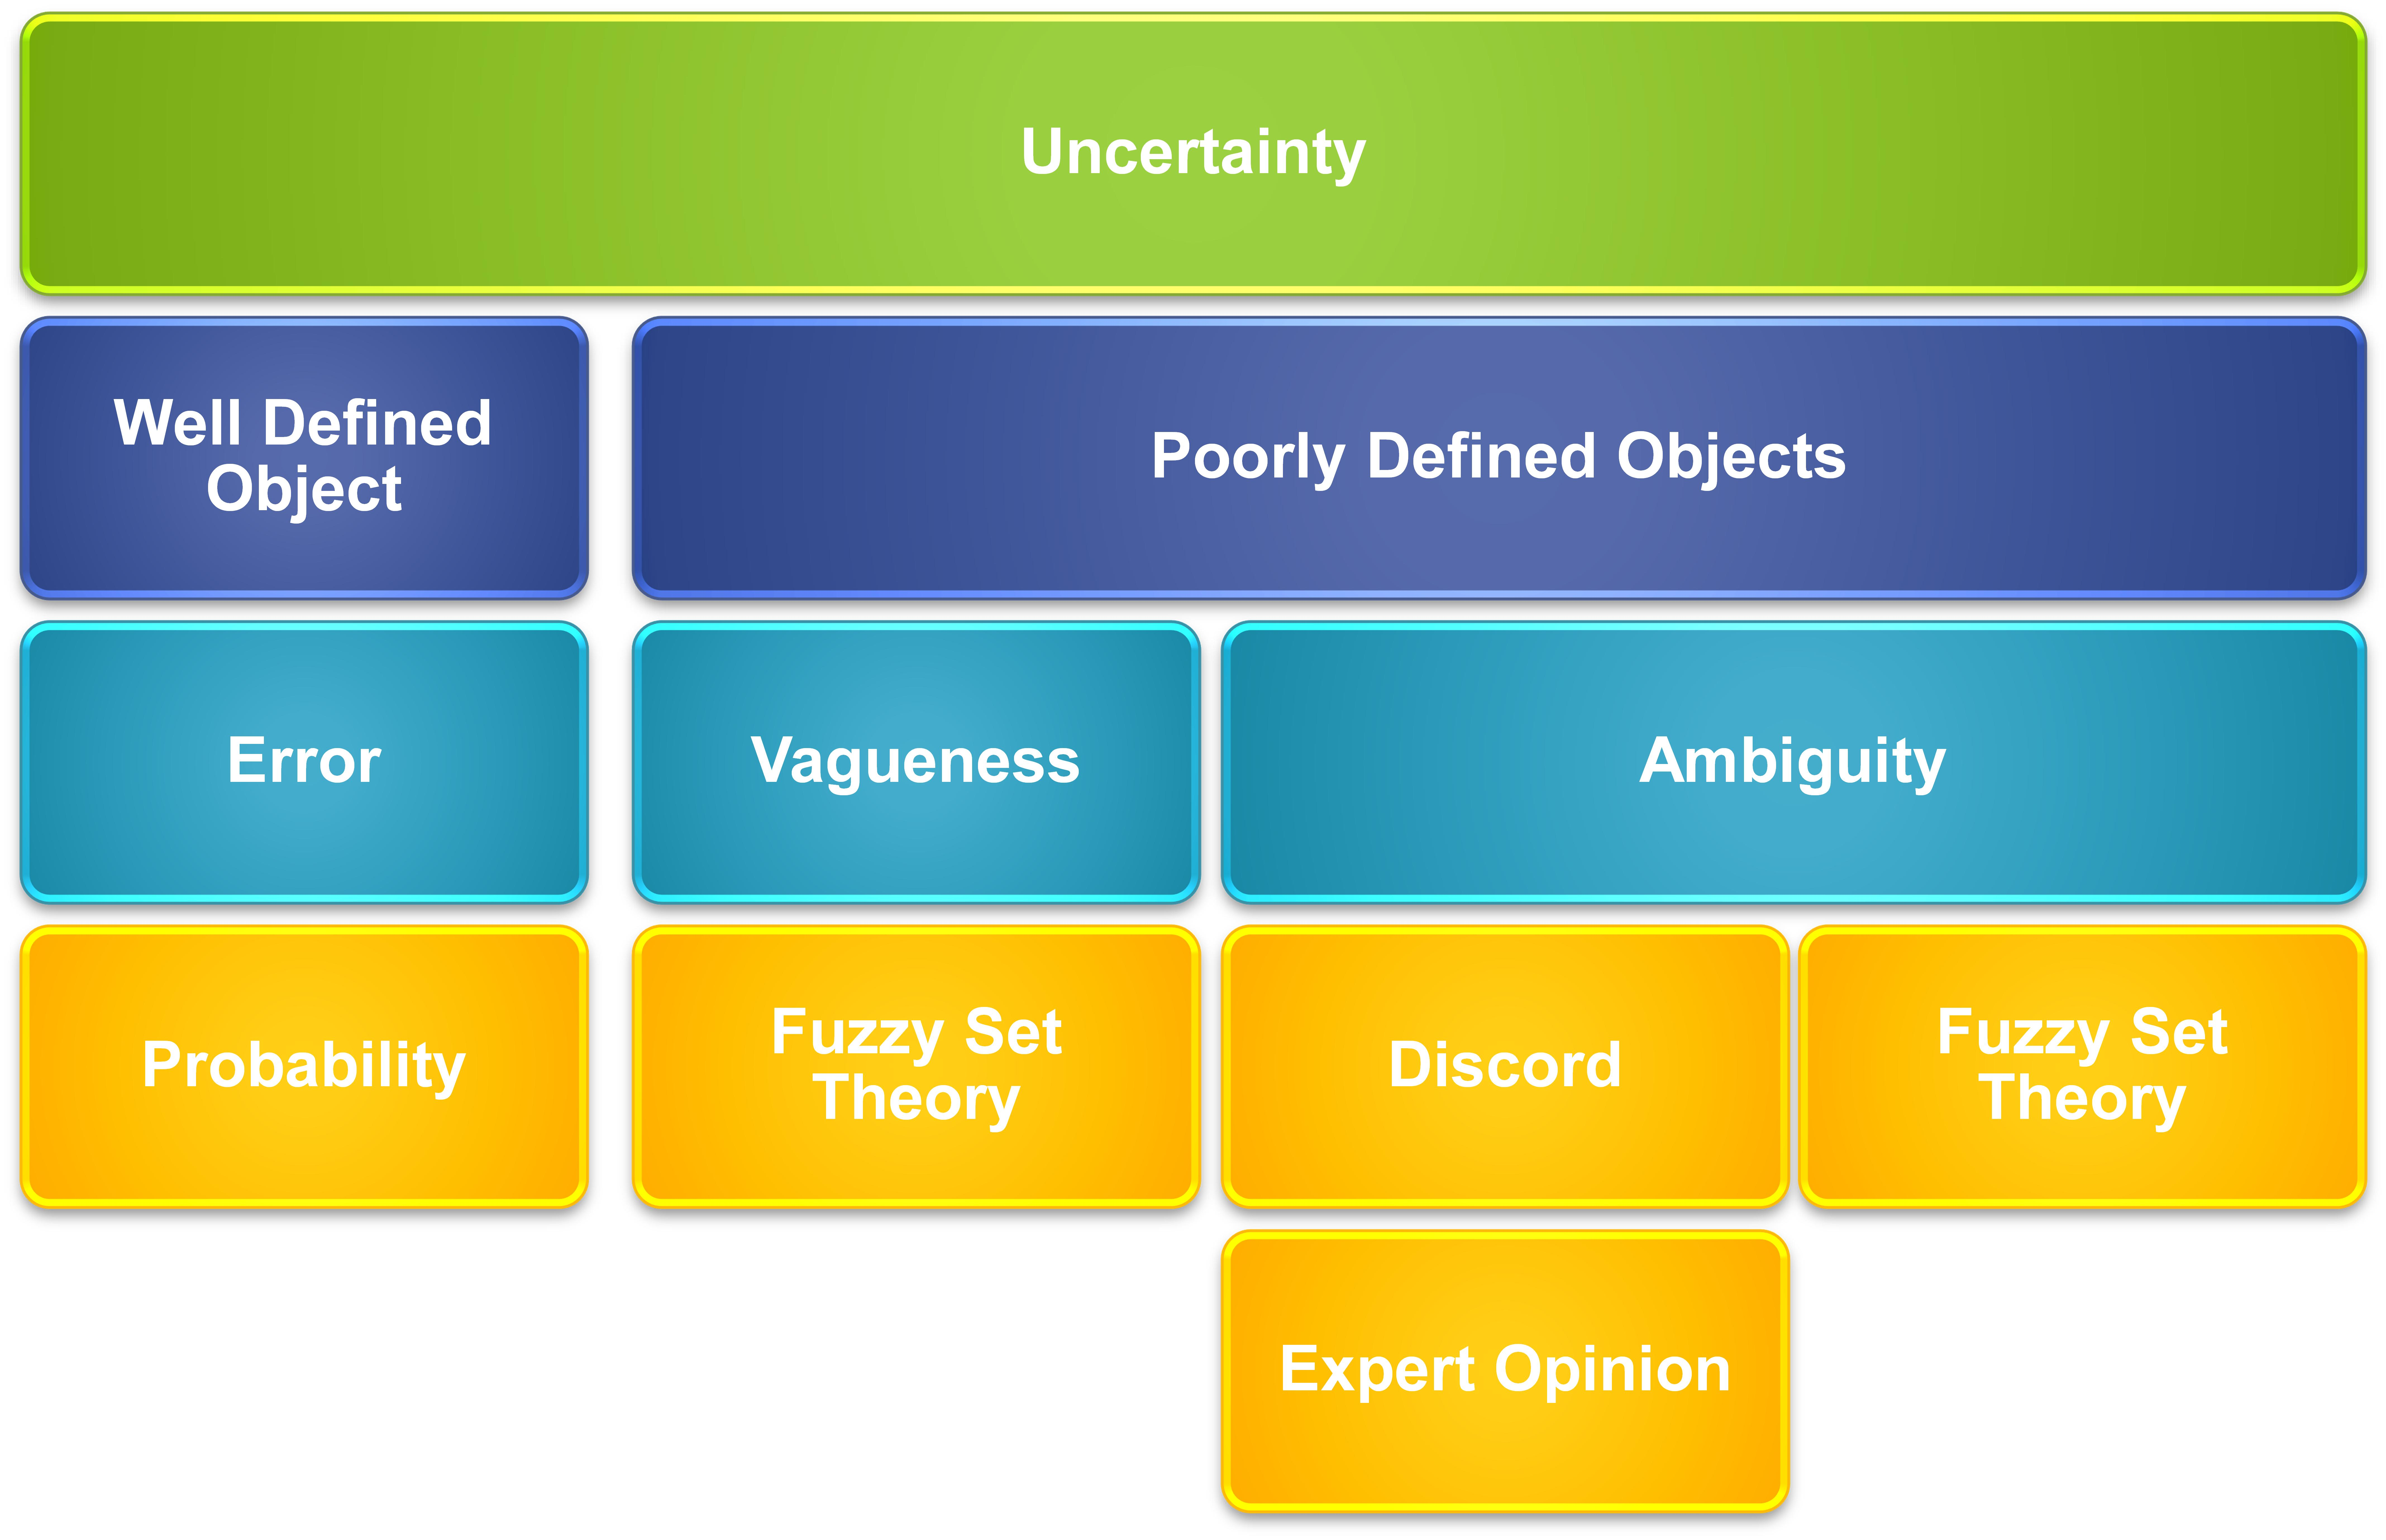
\includegraphics[width=.9\textwidth]{images/uncertainity_type.jpg}
\caption{Types of Uncertainity}
\label{figure:uncertainity_type}
\end{figure}
Real life data analysis shows that the real life data sources do not produce always certain data. Many real life data source produces data with error (correctness is not certain). These types of data is named as uncertain data. Figure \ref{figure:uncertainity_type} shows the uncertainty types of real life dataset. For example location data from GPS sensors mostly produces erroneous data. The correctness of the data is always uncertain. For the uncertainty specialty these types of data gets special attention and concerns to work with. Normal support count is not possible in this type of dataset. This type of database contains data with their corresponding existential probability. That frequent pattern mining of these types of data very much harder. For example, a physician may highly suspicious (but cannot guarantee) that a patient suffers from flu if the patient comes to him having high fever. The uncertainty of such prediction can be expressed in terms of existential probability. For instance, a patient may have a 90\% likelihood of having the flu, and a 20\% likelihood of having a cold regardless of having the flu. or not. So the probability of having flu is .80 and the probability of having cold is .20. So many real life data set may be in between existence and non existence. In these situation an itemset \emph{a\textsubscript{i}} can have own existential probability in \emph{a\textsubscript{i}} between 0 and 1($p_i(0<p_i<1)$). Actually understanding uncertain data is very much tough task but really they exists every where.They come with uncertainity to make us confused in terms of poorly defined object, fuzzy sets, ambiguity, error, inherent probability etc (Figure \ref{figure:uncertainity_type}).\\
There Are many real life scenario where data source always comes with uncertainty. Information gathered from world wide web always inherit uncertainty. For example a system is monitoring user behavior in world wide web. It collects data from different web sites, extract information and analyze. After certain period it finds that one user Mr. X is citizen of country Y. As he/she can work in Y, there must be a probability that Mr. X is citizen of Y. There must be a probability value associate with Mr. X's citizenship. So the data is definitely uncertain. Many sensors produce values with some error like 10\% error from GPS data or temperature reading from cell phones.\\
There is three models of uncertain data in databases.
\paragraph{Attribute Uncertainty}
In this model, every attribute of a tuple has its own probability distribution. For example, if sensor readings are collected for temperature, humidity, precipitation and wind speed then each would be presented with its own probability distribution. Table \ref{table:uncertain_stream_transaction} represents an example of attribute uncertainty.
\paragraph{Correlated Uncertainty}
In this model, several attributes may have a joint probability distribution. For example, most of the time the flu comes with a strong head ache. So these two disease may have come with a joint probability distribution.
\paragraph{Tuple Uncertainty}
In this model, all attributes of a tuple have one joint probability. In table \ref{table:uncertain_stream_transaction}  each items in the tuple has an uncertinity corresponding to it. If the tuple itself has a probability value of existence than it will be tuple uncertainity model.\\
Many approaches has been proposed for finding frequent patterns over uncertain data (U-Apriori ~\cite{u_priori}, UF-growth ~\cite{uf_growth}, UFP-gorwth ~\cite{ufp_growth} etc). As the data existance in the database is not certain then normal support calculation is not easy that makes uncertain data very mistrious. So exact frequent pattern finding makes a huge resource sacrifices. For the improvement many approximate algorithms have been proposed (CUF-growth ~\cite{cuf_growth}, CUF\textsuperscript{*}-growth ~\cite{cuf_growth}, PUF-growth ~\cite{puf_growth}). Most of them suffers producing false positives. False positives are those who are not actually frequent but exists in frequent pattern set.

\subsection{Stream Data}
In real life with enormous use of internet, artificial computerized and artificially intelligent devices (smart phones, tablet pc, cars, smart cards etc) the data source produces a stream millions of data each and every micro seconds. Storing these data in some storage is out of think now a days. But this huge data is very valuable for getting interesting information. Moreover once these data flooded away then can never be found again. The most important property of this kind of dataset is this dataset is unbounded and restless and can not be defined previously how much data will come. Most recent data is most important but old one is not insignificant and can not be ignored. This produces a great challenge for researchers to find interesting information from a continuous data stream.\\
For example with growth of smart phone uses much more applications are hitting each and every seconds. Form these usage and data flood finding user behavior to offer some promotional offer for increasing the sell of online retailer is very tough job. Another example can be the CCTV video footage of traffic camera. That produces a large number of data flood. In this regard any sort of any terrorist activity prediction will be very much significant and necessary information for the government. But for a lot of continuous data makes this a very hard job.\\
Stream data makes the database dynamic as there is no limit of data. To find frequent itemset in data stream several algorithms (~\cite{uncertain_01}, ~\cite{uncertain_02}, ~\cite{uncertain_03}, ~\cite{uncertain_04}, ~\cite{uncertain_05}, ~\cite{uncertain_06}) has been proposed. But most are for handling stream but certain data. The uncertainty property makes mining task more complex and complecated the data stream. FP-streaming ~\cite{suf_growth} and  SUF-growth ~\cite{suf_growth} has been proposed for finding frequent, interesting patterns from uncertain and stream data. But these approaches have to compromise runtime efficiency or correctness. However these SUF-growth ~\cite{suf_growth} is an exact approach to find frequent patterns.
\begin{figure}
\centering
  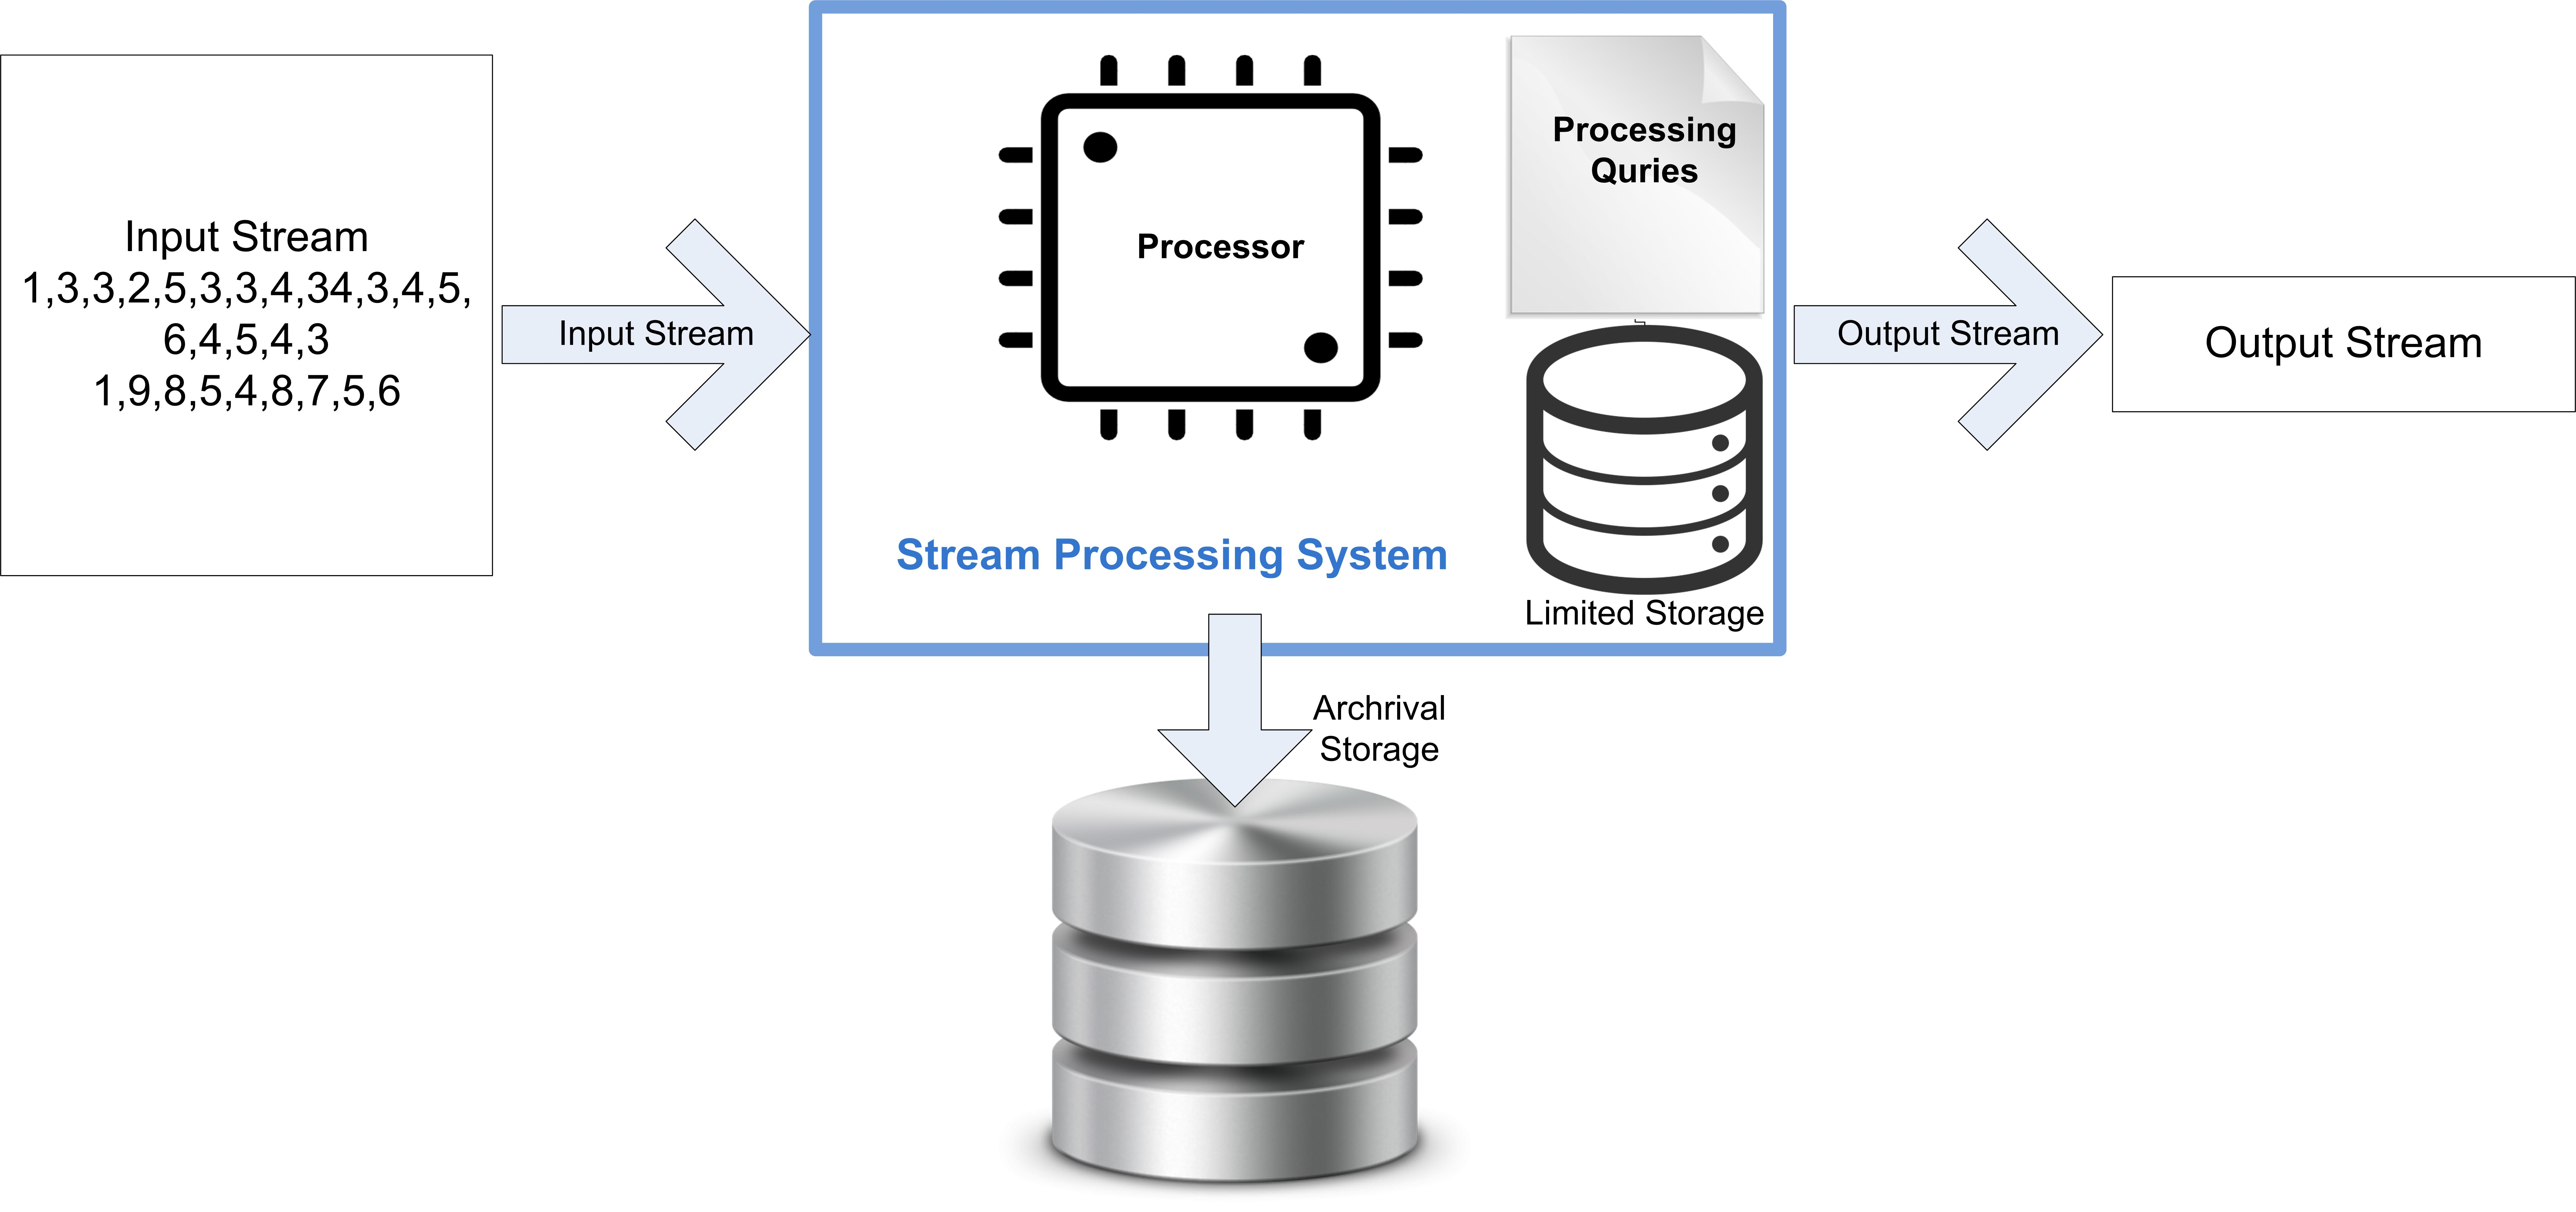
\includegraphics[width=.9\textwidth]{images/stream_data.jpg}
\caption{Types of Uncertainty}
\label{figure:stream_data}
\end{figure}


\section{Motivating Example}
Real life example of data mining.


\section{Aims and Objectives}
Many algorithms has been proposed for mining frequent patterns over certain and uncertain data. Among them in uncertain data mining exact approaches either runitme and the probabilistic models suffers from false positives. More over extraction knowledge from uncertain stream data suffers a lot. The findings are listed briefly below:
\begin{itemize}
	\item Existing algorithms for uncertain data mining suffers either from runtime compromise or the compactness of data storage
	\item In probabilistic uncertain data modeling approach suffers from huge false positives with the frequent itemset.
	\item The proposed data structure in existing approaches for mining uncertain stream data suffers from memory optimization.
	\item Reduction of huge false positives from candidate frequent itemset suffers from runtime inefficiency.
\end{itemize}
To overcome these problems we have follow some objectives. They are given below:
\begin{itemize}
	\item A complete new efficient, robust, scalable approach work with new data structure that will memory efficient.
	\item Memory and runtime efficient data-structure for both uncertain dynamic database nad static databases.
	\item Attach any meta-data with each items of transaction that will make the runtime storage compact as much as possible.
	\item Most recent data is more significant - with this characteristic storing as much as recent data that has more probability to be important.
	\item Giving users the opportunity to keep her/his recent information data as she/he wishes.

\end{itemize}


\section{Our Contribution}
Our key contributions of this paper are given below:
\begin{itemize}
\item We have introduced an prefix value for each items in a transaction which always maintain upper bound of probability. That helps us to make compact pattern tree construction.
\item A new approach \emph{US-tree} that is very much compact and very memory efficient
\item A new mining algorithm \emph{USFP-growth} that is very efficient and reduce mining time surprisingly.
\item 
\end{itemize}


\section{Thesis Organization}
We have carried out the thesis work to consummate the objectives. An outline of rest of the chapters is provided as follows:
\paragraph{Chapter 2}
Describes the necessary background study and existing approaches.
\paragraph{Chapter 3}
Provides the details of our proposed approach with required analysis.
\paragraph{Chapter 4}
Presents the results of experimental results in detail with comparison and analysis.
\paragraph{Chapter 5}
Shows several real life applications for our proposed approach and ends the thesis with a brief conclusion and future scopes.
%\end{document}